\documentclass{beamer}
\usetheme{Frankfurt}
\usecolortheme{whale}

%%%%%%%%%%%%%%%%%%%%%%%%%%%%% packages %%%%%%%%%%%%%%%%%%%%%%%%%%%%%
\usepackage{graphicx}
\usepackage{booktabs}
\usepackage{xmpmulti}
\usepackage{appendixnumberbeamer}
\usepackage{booktabs}
\usepackage{listings}
\usepackage{xcolor}

\definecolor{codegreen}{rgb}{0,0.6,0}
\definecolor{codegray}{rgb}{0.5,0.5,0.5}
\definecolor{codepurple}{rgb}{0.58,0,0.82}
\definecolor{backcolour}{rgb}{0.95,0.95,0.92}

\lstdefinestyle{mystyle}{
    backgroundcolor=\color{backcolour},   
    commentstyle=\color{codegreen},
    keywordstyle=\color{magenta},
    numberstyle=\tiny\color{codegray},
    stringstyle=\color{codepurple},
    basicstyle=\ttfamily\footnotesize,
    breakatwhitespace=false,         
    breaklines=true,                 
    captionpos=b,                    
    keepspaces=true,                 
    numbers=left,                    
    numbersep=5pt,                  
    showspaces=false,                
    showstringspaces=false,
    showtabs=false,                  
    tabsize=2
}

\lstset{style=mystyle}


%%%%%%%%%%%%%%%%%%%%%%%%%%%%% adjust template %%%%%%%%%%%%%%%%%%%%%%%%%%%%%
% Remove navigation icons
\setbeamertemplate{navigation symbols}{}
% Show slide numbers
\setbeamertemplate{footline}[frame number]
% Show index
\AtBeginSection[]{
  \begin{frame}{Next section}
    \tableofcontents[currentsection, hideallsubsections]
  \end{frame}
}

%%%%%%%%%%%%%%%%%%%%%%%%%%%%% Metadata %%%%%%%%%%%%%%%%%%%%%%%%%%%%%
\title{CLI, HPC workshop}
\subtitle{}
\date{24-11-2026}
\author{Doğukan Bayraktar}

\begin{document}

%%%%%%%%%%%%%%%%%%%%%%%%%%%%% Title Slide %%%%%%%%%%%%%%%%%%%%%%%%%%%%%
\begin{frame}
    \titlepage
    
\includegraphics[height=.1\textheight]{images/logo/umcu.png}
    
\includegraphics[height=.1\textheight]{images/logo/mmbbioit.png}
\end{frame}

%%%%%%%%%%%%%%%%%%%%%%%%%%%%% %%%%%%%%%%%%%%%%%%%%%%%%%%%%%
\section{Commandline basics}




%%%%%%%%%%%%%%%%%%%%%%%%%%%%% %%%%%%%%%%%%%%%%%%%%%%%%%%%%%
\section{What is the HPC}

\begin{frame}{What is the HPC?}
  \begin{columns}[T] % [T] aligns tops; use [c] or [b] for center/bottom
    \begin{column}{0.48\textwidth}
        \begin{itemize}
            \item HPC stands for High-performance computing.
            \item The HPC is a cluster of computers that work together as a single system
            \item The computers run Rocky Linux
            \item It is managed through SLURM.
        \end{itemize}
    \end{column}

    \begin{column}{0.48\textwidth}
      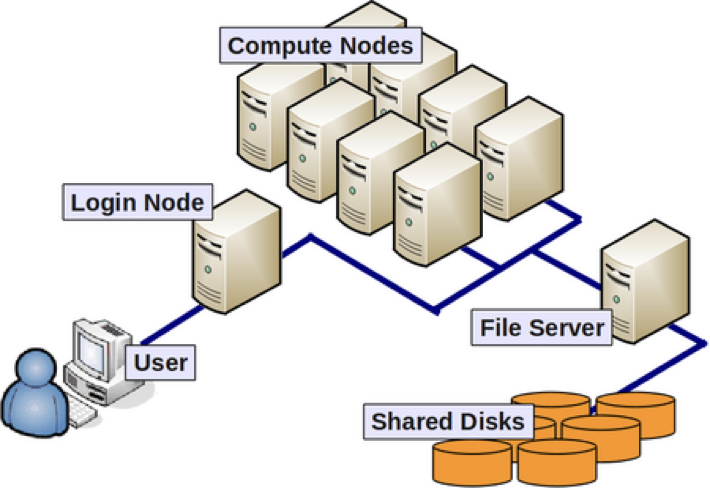
\includegraphics[width=\linewidth]{images/cluster_draw.png}
    \end{column}
  \end{columns}
\end{frame}

%%%%%%%%%%%%%%%%%%%%%%%%%%%%%  %%%%%%%%%%%%%%%%%%%%%%%%%%%%%
\begin{frame}{Hardware: CPU}

CPU stands for Central Processing Unit. This is the component that
processes everything you do on your computer.

On my umc laptop the specs associated with this component are:
\begin{itemize}
    \item \textbf{Processor Name}: Apple M3
    \item \textbf{Processor Speed}: 4.06 GHz
    \item \textbf{Number of Processors}: 1
    \item \textbf{Total number of Cores}: 8
\end{itemize}

So, I have a processor with 8 "cores". This means that my processor can
do 8 distinct computations at the same time.
\end{frame}

%%%%%%%%%%%%%%%%%%%%%%%%%%%%%  %%%%%%%%%%%%%%%%%%%%%%%%%%%%%
\begin{frame}{Hardware: Data Storage}
There are 2 options for built-in data storage:
\begin{itemize}
    \item HDD: Hard Disk Drive (spinning)
    \item SSD: Solid State Drive
\end{itemize}
Measured in bytes, usually Gigabytes (GB) or Terabytes (TB). 

\vspace{\baselineskip}
E.g. my UMC laptop has 560 GB of storage.
\end{frame}

%%%%%%%%%%%%%%%%%%%%%%%%%%%%%  %%%%%%%%%%%%%%%%%%%%%%%%%%%%%
\begin{frame}{Hardware: Memory}
Memory is a small amount of volatile or temporary information storage.
This is distinct from the data storage we discussed in the previous
point. It is an essential component of any computer, as this is where
data is stored when some computation is being performed on it.

\vspace{\baselineskip}
E.g. my UMC laptop has 8 GB of memory. 
\end{frame}

%%%%%%%%%%%%%%%%%%%%%%%%%%%%%  %%%%%%%%%%%%%%%%%%%%%%%%%%%%%
\begin{frame}{Compute on the HPC cluster}
\begin{itemize}
    \item 57 compute-CPU-nodes
    \item 2 login/submission servers
    \begin{itemize}
        \item hpcs05
        \item hpcs06
    \end{itemize}
    \item 2 transfer servers
    \begin{itemize}
        \item hpct04
        \item hpct05
    \end{itemize}
    \item and more...
\end{itemize}
\end{frame}

%%%%%%%%%%%%%%%%%%%%%%%%%%%%%  %%%%%%%%%%%%%%%%%%%%%%%%%%%%%
\begin{frame}{Cluster CPU node specs}
\centering\small
\setlength{\tabcolsep}{4pt}
\begin{tabular}{@{}lrrrrrrr@{}}
\toprule
\textbf{Nodes} & \textbf{\#} & \textbf{Mem} & \textbf{CPUs} & \textbf{C/CPU}
  & \textbf{Cores} & \textbf{MHz} & \textbf{TMP} \\
\midrule
n0061              & 1  & 256  & 2 & 12 & 24 & 2500 & 1000 \\
n0062              & 1  & 384  & 2 & 18 & 36 & 2133 & 2000 \\
n0063--n0080$^*$   & 16 & 384  & 2 & 18 & 36 & 2300 & 2000 \\
n0065              & 1  & 1023 & 4 & 12 & 48 & 2300 & 2000 \\
n0081--n0095$^\dagger$ & 11 & 384 & 2 & 20 & 40 & 2400 & 2000 \\
n0087--n0090       & 4  & 384  & 2 & 20 & 40 & 2600 & 2000 \\
n0103--n0123       & 20 & 384  & 2 & 20 & 40 & 3100 & 1300 \\
n0134--n0136       & 3  & 1024 & 2 & 16 & 32 & 2800 & 1500 \\
\midrule
\textbf{Total}     & \textbf{57} & & & & \textbf{2172} & & \\
\bottomrule
\end{tabular}
\par\medskip
{\footnotesize $^*$excl.\ n0065 \quad $^\dagger$excl.\ n0087--n0090 \quad Mem/TMP in GB}
\end{frame}


%%%%%%%%%%%%%%%%%%%%%%%%%%%%%%%%%%%%%%%%%%%%%%%%%%%%%%%%%%
\section{How to connect to the HPC}
%%%%%%%%%%%%%%%%%%%%%%%%%%%%%%%%%%%%%%%%%%%%%%%%%%%%%%%%%%
\begin{frame}{Connect with SSH}
Secure Shell Protocol (SSH) is a cryptographic network protocol for
operating network services securely over an unsecured network.

Its most notable applications are remote login and command-line execution.
\end{frame}

\begin{frame}[fragile]{Creating a SSH key for HPC usage}

\begin{lstlisting}[]
mkdir ~/.ssh
cd ~/.ssh
ssh-keygen -t ed25519 -C "HPC" -f ~/.ssh/id_ed25519_hpc
\end{lstlisting}

When prompted,  enter a strong, secure passphrase.
\par\medskip
This will create two files: id\_ed25519\_hpc, and id\_ed25519\_hpc.pub.
\par\medskip
Please mail the id\_ed25519\_hpc.pub file to hpcsupport@umcutrecht.nl

\end{frame}

\begin{frame}[fragile]{Setting up your ssh config}

Open ~/.ssh/config

\begin{lstlisting}[]
# usage : ssh gw2hpcs05
Host gw2hpcs05
HostName hpcs05.op.umcutrecht.nl
User dbayraktar
ProxyJump hpcgw

# usage : ssh gw2hpcs06
Host gw2hpcs06
HostName hpcs06.op.umcutrecht.nl
User dbayraktar
ProxyJump hpcgw
\end{lstlisting}

\end{frame}

\begin{frame}{Using On-demand}
  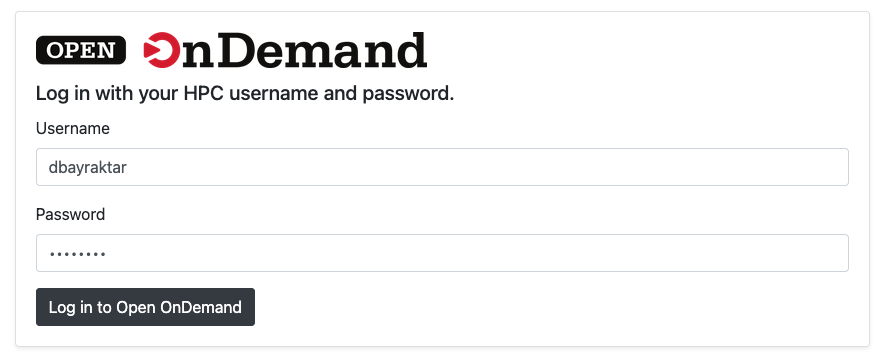
\includegraphics[width=\linewidth]{images/ondemand1.png}

  \begin{itemize}
    \item hpcs05.op.umcutrecht.nl
    \item hpcs06.op.umcutrecht.nl
  \end{itemize}
\end{frame}


%%%%%%%%%%%%%%%%%%%%%%%%%%%%%%%%%%%%%%%%%%%%%%%%%%%%%%%%%%
\section{How to make use of the HPC}
%%%%%%%%%%%%%%%%%%%%%%%%%%%%%%%%%%%%%%%%%%%%%%%%%%%%%%%%%% 
\begin{frame}{Who makes use of the HPC?}
	\begin{itemize}
		\item University Medical Center Utrecht
		\begin{itemize}
			\item Division Biomedical
			\item Division Cardiology \& Pulmonology
			\item Division Imaging
			\item Division Internal Medicine
			\item Julius Center
			\item Division Laboratories \& Pharmacy
			\item Division Neuroscience
		\end{itemize}
		\item Utrecht University
		\begin{itemize}
			\item Science Faculty, Department of Information and Computing Sciences
			\item Science Faculty, Department of Biology
		\end{itemize}
		\item Hubrecht Institute
		\item Princess Máxima Center for Pediatric Oncology
	\end{itemize}
\end{frame}

%%%%%%%%%%%%%%%%%%%%%%%%%%%%%  %%%%%%%%%%%%%%%%%%%%%%%%%%%%%
\begin{frame}{SLURM and submitting jobs}
  \begin{columns}[T] % [T] aligns tops; use [c] or [b] for center/bottom
    \begin{column}{0.48\textwidth}
    \begin{itemize}
        \item SLURM is a cluster management and job scheduling tool. Its used to manage user-accounts, jobs, and logs.
        \item Never run an analysis on the login/submission nodes or the transfer nodes.
        \item If you want to perform an analysis you request resources through SLURM and then gain acces to a compute node that has those resources.
    \end{itemize}
    \end{column}

    \begin{column}{0.48\textwidth}
      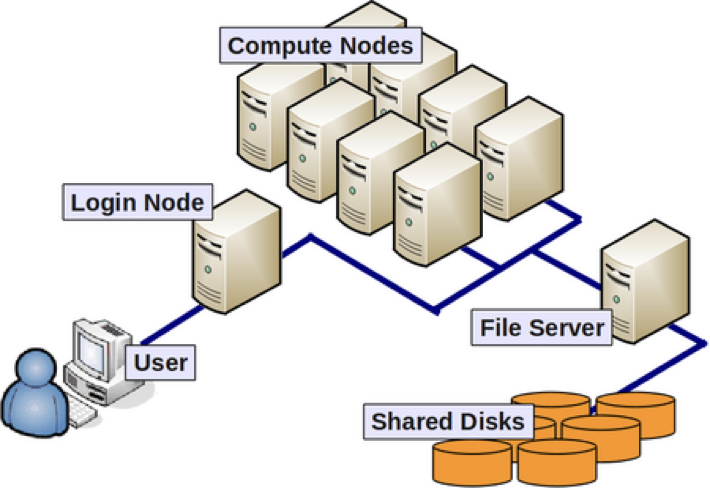
\includegraphics[width=\linewidth]{images/cluster_draw.png}
    \end{column}
  \end{columns}
\end{frame}

%%%%%%%%%%%%%%%%%%%%%%%%%%%%%  %%%%%%%%%%%%%%%%%%%%%%%%%%%%%
\begin{frame}[fragile]{Using srun for interactive sessions}
Requesting an interactive job:
\begin{lstlisting}[]
srun --gres=tmpspace:50G --mem=4G --time=24:00:00 -c 4 --pty bash
\end{lstlisting}
\end{frame}

%%%%%%%%%%%%%%%%%%%%%%%%%%%%%  %%%%%%%%%%%%%%%%%%%%%%%%%%%%%

\begin{frame}[fragile]{Using sbatch to submit scripts}

Command:
\begin{lstlisting}[]
sbatch assemble.sh
\end{lstlisting}

Script content:
\begin{lstlisting}[]
#!/bin/bash
#SBATCH --job-name=unicycler
#SBATCH --output=output.log
#SBATCH --error=error.log
#SBATCH --cpus-per-task=16
#SBATCH --time=72:00:00
#SBATCH --gres=tmpspace:100G
#SBATCH --mem=32G

# Go through all R1 fastq files in the current directory
for r1_file in *_R1*.fastq*; do
    # Get the name of the paired read
    r2_file="${r1_file/_R1/_R2}"
    ...
\end{lstlisting}
\end{frame}

\begin{frame}[fragile]{Checking in on jobs/queue}
  \begin{lstlisting}[]
  sqeueu

  squeue -u dbayraktar

  squeue -A dla_mm
  \end{lstlisting} 
\end{frame}

%%%%%%%%%%%%%%%%%%%%%%%%%%%%%  %%%%%%%%%%%%%%%%%%%%%%%%%%%%%
\begin{frame}{Requesting resources does not equal using them}
  When you request resources they become available in your session on the
  compute node. You are now occupying these resources and others cannot
  use them. To actually make use of them you have to tell the tool you
  are using that those resources are available. Usually by passing a
  commandline flag suchs as \texttt{-{}-threads}  \texttt{-{}-mem}. Also consider that
  efficiency reaches a platau when using a lot of threads. E.G. two
  people digging a hole will be much faster than one. But twenty people
  digging a hole most of them will be standing around doing nothing.
    
\end{frame}

\begin{frame}[fragile]{Checking actual resource usage}
  \begin{lstlisting}[]
  seff <jobid>
  \end{lstlisting}
\end{frame}

\end{document}
